\Chapter{Kamerapozíció becslése a virtuális térben}

Ahhoz, hogy a virtuális tér elemeit a valós térből kapott képre rá lehessen illeszteni, meg kell tudni becsülni, hogy a kamera abban hol helyezkedik el.
Erre többféle lehetőség is adódik.
A fejezetben ezek áttekintésére kerül sor.

\Section{Markerek}

A markerek olyan, fizikális jelölő pontok, amelyeket képfeldolgozási módszerekkel, a\-rány\-lag nagy megbízhatósággal be lehet határolni a kameraképen.
Az AR/VR technológiák fejlődésével az egyszerűbb, szembetűnő markerektől fokozatosan jutott el a technológia a betanítható markerekig (illetve a marker nélküli megoldásokig).
A következő szakaszokban a két jellegzetes megközelítés kerül részletezésre.

\SubSection{Klasszikus markeres megoldások}

A kiterjeszetett valóság fontos eszköze a markerek, így azok használata jól támogatottnak mondható. Számos nyílt forráskodú könytár rendelkezésre áll a klasszikus értelemben vett markerekből.

\bigskip

\noindent \textbf{Vonalkód, QR-kód}

\medskip

A vonalkódokat és a QR kódokat az információ tároláson túl használhatjuk pozíció becslésére is.
A QR-kód neve \textit{Quick Response}-t, vagyis gyors választ jelent.
Ez egy kétdimenziós kód. Működésében nagyon hasonlít a vonalkódhoz, gyakorlatilag annak egy fejlettebb változatáról van szó.
Míg egy vonalkód esetében jellemzően 13 számjegy kerül tárolásra, addig a QR kód akár 7000 számjegyet és 4300 alfanumerikus karaktert tud kódolni, például egy weboldal URL-jét \cite{tiwari2016introduction}.
Ezekre láthatunk egy-egy példát \aref{fig:barcode}. ábrán.

\begin{figure}[htp]
    \centering
   	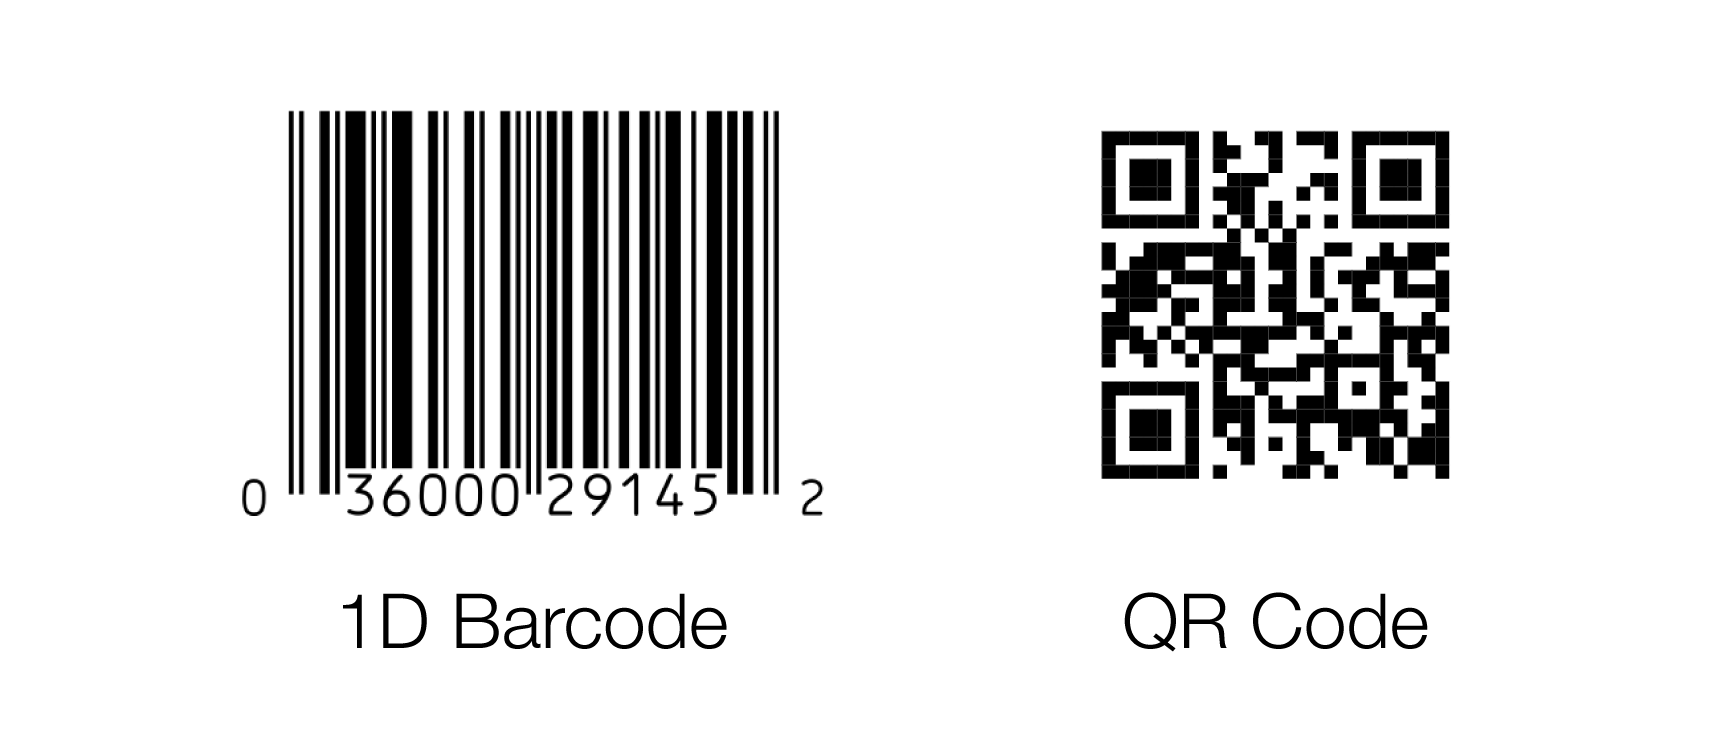
\includegraphics[scale=0.25]{images/qr_bar.png}
	\caption{Példa vonalkódra és QR-kódra}
	\label{fig:barcode}
\end{figure}

\bigskip

\noindent \textbf{„Keretes” markerek}

\medskip

Az ilyen típusú markerek két részből állnak; egy fekete keretből, ami a felismerést segití és egy belső mintából. A belső minta lehet kép, egyedi bináris minta, amely azonosítja a markert, információt hordoz.

A keret fontos szerepet tölt be, hisz egy fekete téglalapot/négyzetet viszonylag egyszerűen és gyorsan fel lehet ismerni egy képen, meghatározni annak pozícióját a kamerához képest, sarok pontjait, a középpontját.

Ilyen típusú marker például az \textit{ARToolKit} marker (amelynél középen egy kép van, ami bináris képként lesz kezelve), \textit{ARTag}, \textit{AprilTag} és az \textit{ArUco}.

Kombinálni is szokták az egyszerűbb markereket: a QR-kódot és a kerettel rendelkező markereket, vagy a QR kód van a keret belsejében vagy pedig a QR kód közepén szerepel például egy ArUco marker vagy egy kép (mint például a \textit{VuMark} esetén).
Ezekre láthatunk példákat \aref{fig:markerek}. ábrán.

\begin{figure}[htp]
    \centering
   	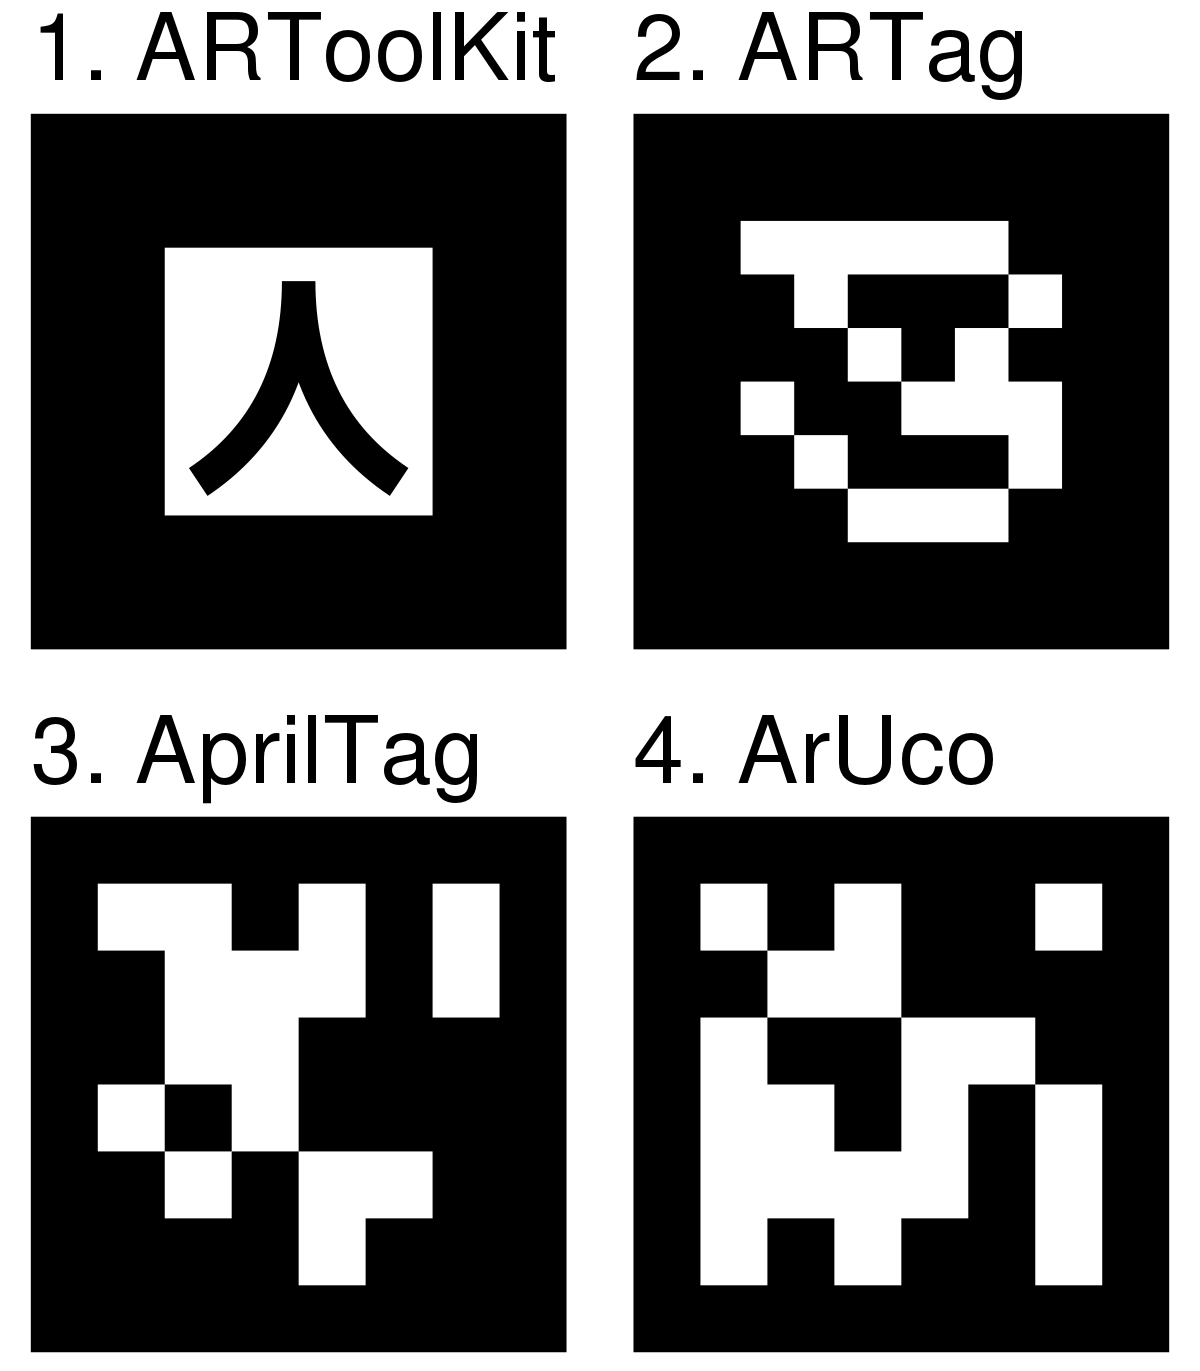
\includegraphics[scale=0.25]{images/markerek.png}
	\caption{ArToolKit, ARTag, AprilTag, ArUco}
	\label{fig:markerek}
\end{figure}

\SubSection{Betanítható markerek}

A kiterjesztett valóság technikai fejlődéssel a markerek is bonyolultabbá váltak, lehetőség nyílt hétköznapi tárgyak, épületek és egyéb valós objektumok markerként történő kezelésére.

Természetesen ezek detektálása nehezebb, illetve betanítást igényel.

Léteznek továbbá úgynevezett marker nélküli (\textit{markerless}) AR alkalmazások is, amelyekben a szenzorok felmérik környezetet és megfelelő helyre pozicionálják a megjelenítendő objektumot/objektumokat. Egy ismert példa erre a földrajzi koordináták felhasználásával működő \textit{Pokemon GO} játék.

\Section{Inerciális szenzorok}

A fejlettebb telefonokban található inerciális szenzorok fontosak a kiterjeszett valóság felhasználásával készült alkalmazások müködtetéséhez.

Az inerciális szenzorok gyorsulásérzékelőkből és giroszkópokból állnak, minél nagyobb a számuk, annál pontosabb eredményeket képesek biztosítani.

Az inerciális szenzorokkkal a telefon térbeli helyzetének és annak változára vonatkozó adatokat kaphatunk meg.

Az accelerométer a telefon helyzetének változását méri a $x$, $y$ és $z$ tengelyeket alapul véve.

A telefonokban található giroszkóp (vagy röviden \textit{gyro} szenzor) a gyorsulásmérő egy fejlettebb verziója.
Míg accelerometer tengely alapú elmozdulást mér, addig a giroszkóp az acceletométert felhasználva minden apró változást érzékel. Pontosabb adatokat kaphatunk vele.
\Aref{fig:inertial}. ábrán láthatjuk, hogy például hogyan néz ki egy ilyen szenzor.

\begin{figure}[htp]
    \centering
   	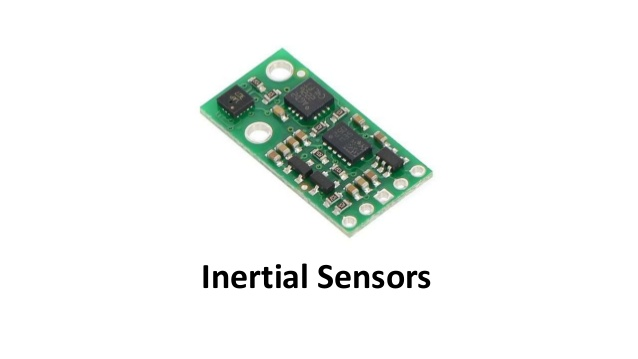
\includegraphics[scale=3]{images/inertial.jpg}
	\caption{inerciális szenzor}
	\label{fig:inertial}
\end{figure}

\Section{Az Aruco marker használata}

Az \textit{ArUco} (\textit{Augmented Reality University of Cordoba}) markereket 2014-ben fejlesztette ki kollégáival S. Garrido-Jurado Spanyolországban \cite{avola2016practical}.
Az ArUco könyvtár OpenCV alapú, nyílt forráskódú, C++ nyelvű függvénykönyvtár.
Ar ArUco markerek két részből állnak: egy fekete keretből és az egyedi bináris mintából, ami azonosítja a markert (mint ahogy például \aref{fig:kep}. ábrán látható).

Alapvetően az OpenCV-s támogatottsága miatt került kiválasztásra a dolgozatban felvetett kamerapozíció becslési problémákhoz. A detektálást számos beépített függvény segíti \cite{garrido2018opencv}.

\begin{figure}[htp]
    \centering
   	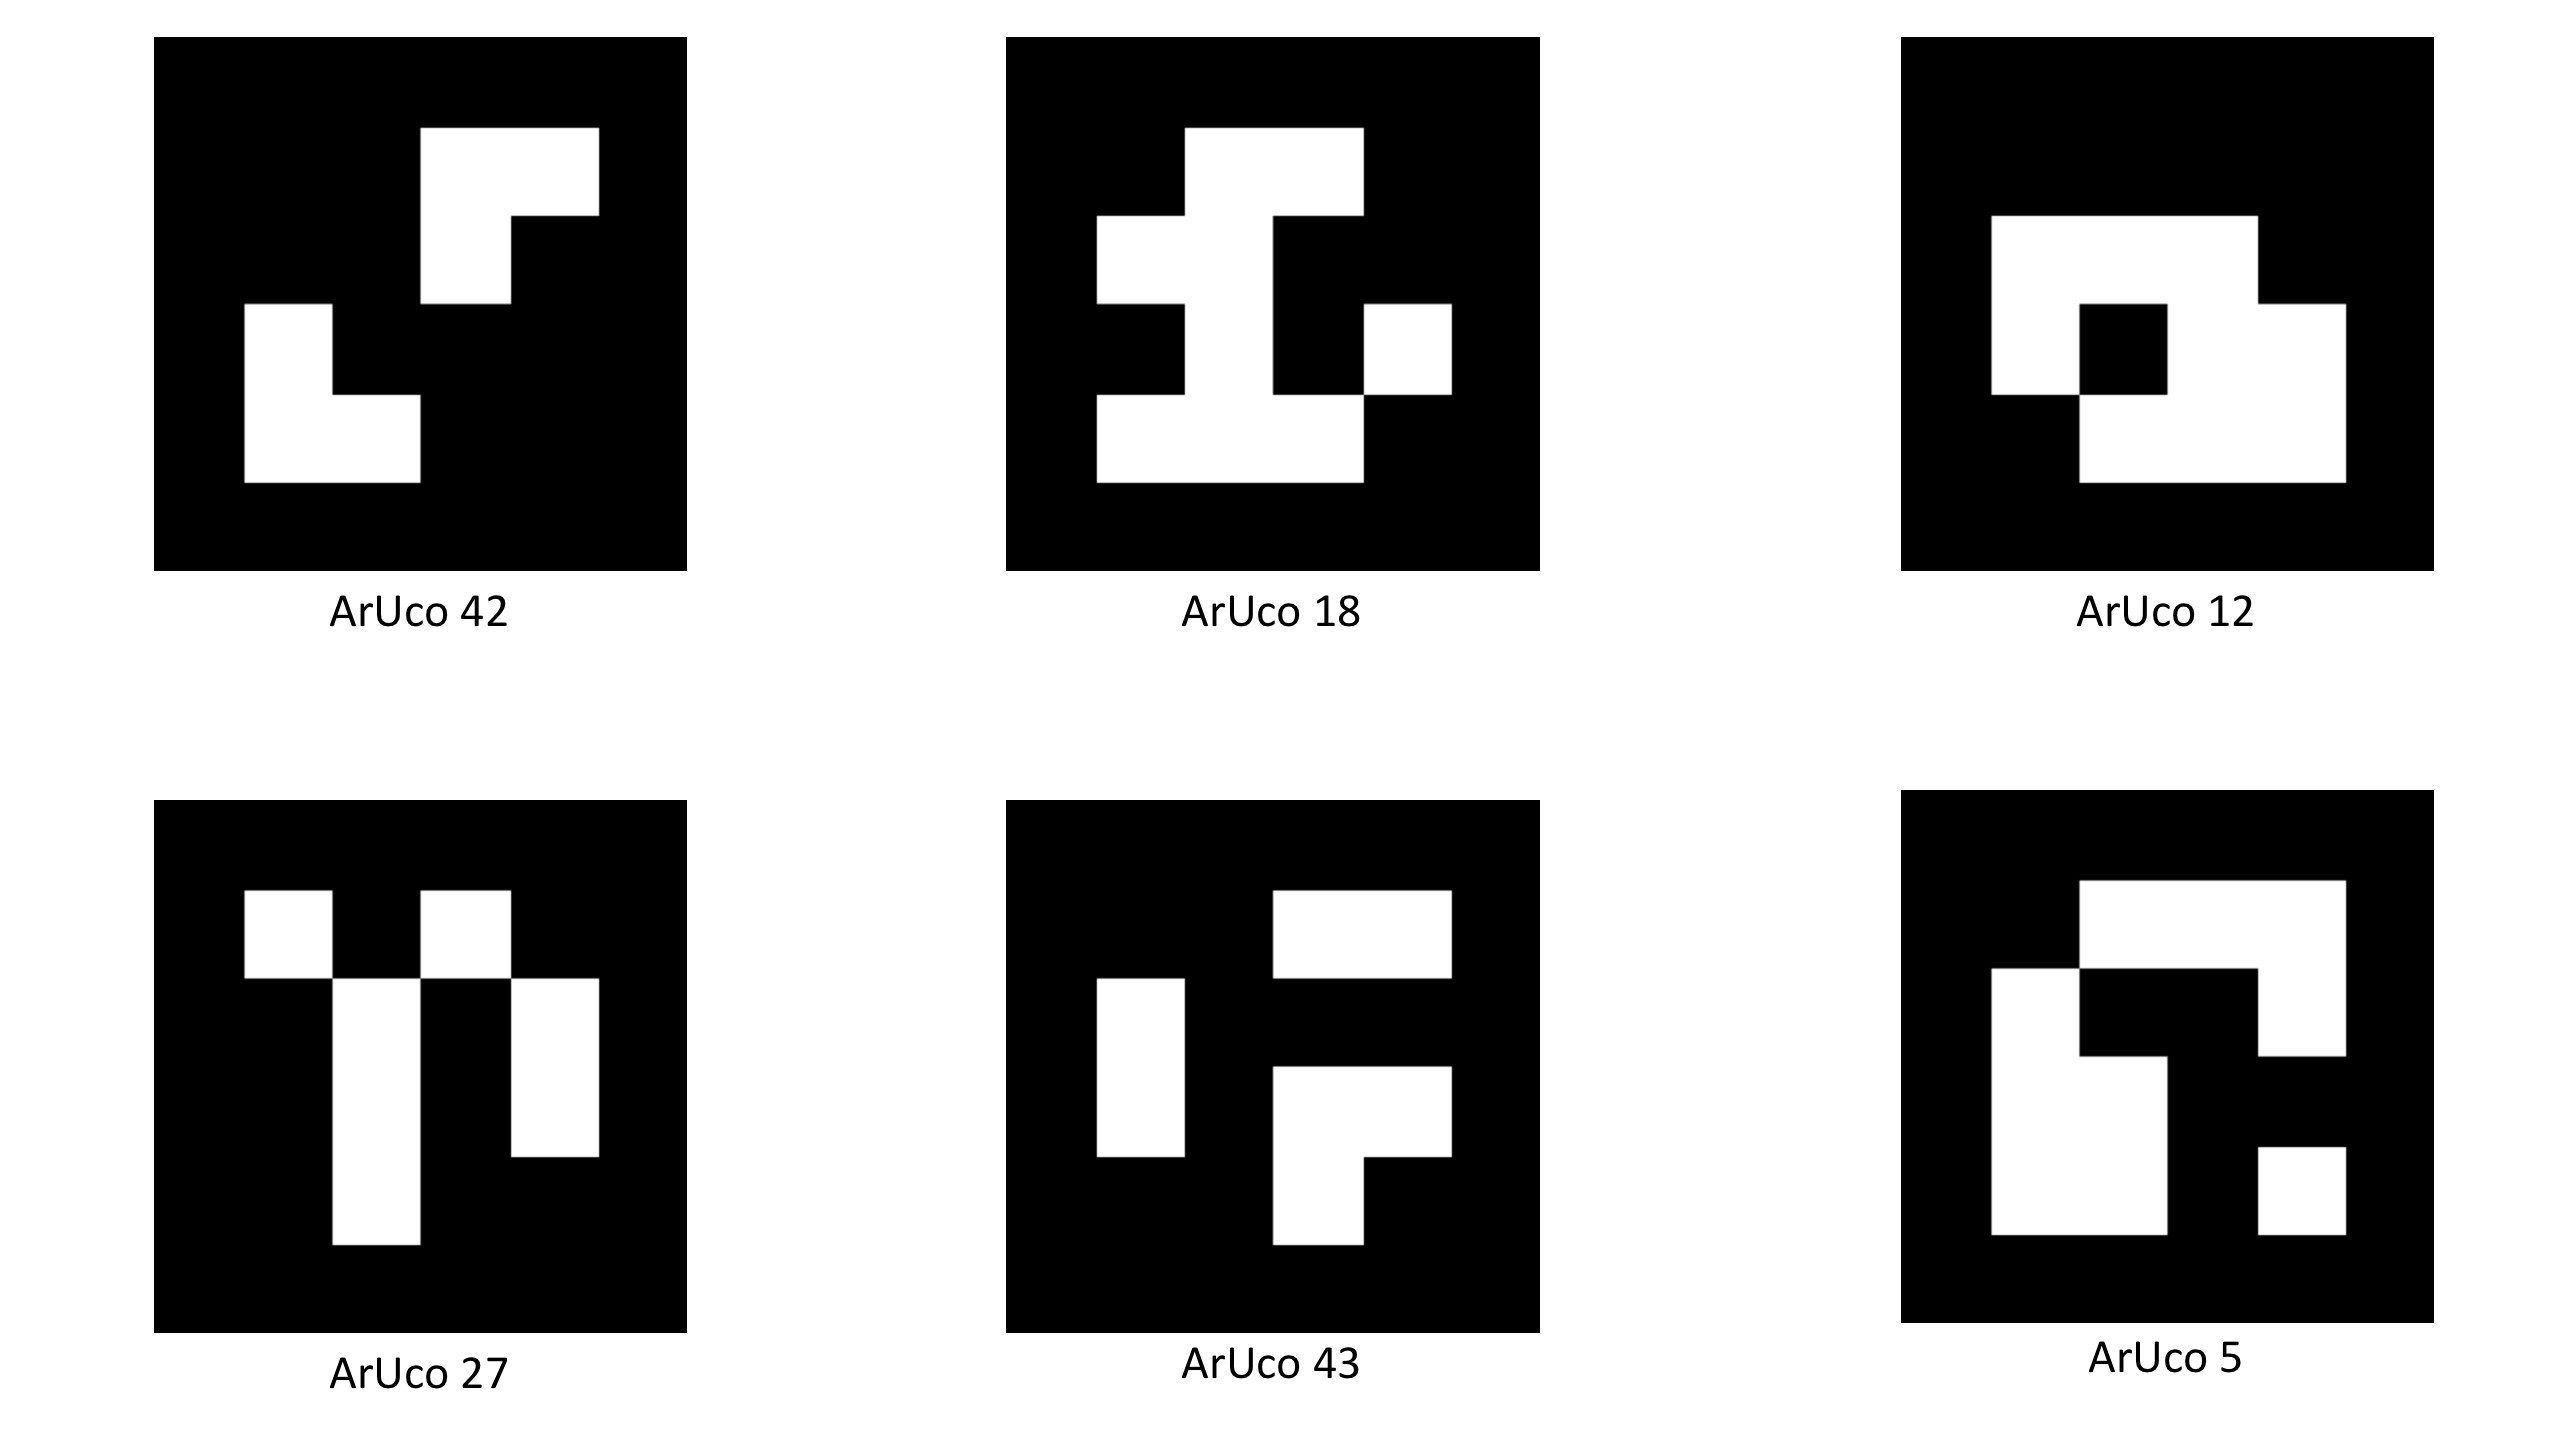
\includegraphics[scale=0.4]{images/kep.png}
	\caption{Aruco markerek a $4 \times 4$-es könyvtárból}
	\label{fig:kep}
\end{figure}

\SubSection{Típusai, használati módok}

Az ArUco markerekhez különböző könyvtárak érhetőek el, amelyek a marker méretében (szükséges bitek száma), belső minta oszlop és sor számában (az oszlop és sor szám mindig megegyezik) és az elérhető azonosítók számában térnek el.
A bináris minta $4 \times 4$-től a $7 \times 7$ bitig terjed (amelybe nem számít bele a keret).

Minél bonyolultabb egy minta, és minél nagyobb annál nehezen felismerni, ezért a \texttt{DICT\_4X4\_100} használata tünt megfelelő választásnak.

Ennél a \texttt{\_4x4} a bitek számát, a \texttt{100} pedig a könyvtárban lévő markerek azonosítóit jelöli.
Ez azt jelenti, hogy az azonosítók 0 és 99 között vannak.

\SubSection{Kamera kalibrálása}

% TODO: https://medium.com/@aliyasineser/aruco-marker-tracking-with-opencv-8cb844c26628

A kamera kalibrációjához $6 \times 9$-es sakktábla mintát használtam (\ref{fig:calibration}. ábra). (A külső sáv nem számolandó bele, az a felismerést könnyíti, a belső minta számít.)

\begin{figure}[htp]
	\centering
	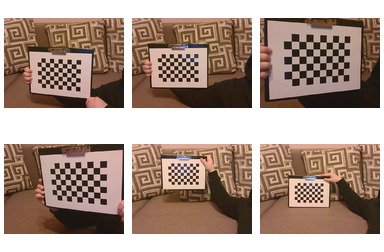
\includegraphics[scale=1]{images/calibration.jpg}
	\caption{Kalibráláshoz használt képek közül néhány}
	\label{fig:calibration}
\end{figure}

A kalibráció eredményességéhez a négyzeteknek szabályosnak, egyformának kell lenniük és fontos, hogy a nyomtatás során a minta ne torzuljon el, ne legyen átméretezve.

A pontosság növelése érdekében a képeket érdemes minél változatosabb szögben és távolságból elkészíteni. Valamint ügyelni kell arra, hogy a lap egyenes legyen tartva, ezért célszerű megfelelő támaszt használni hozzá.

A kalibráció során kapjuk meg a későbbiekben nélkülözhetetlen együttható (kamera) mátrixot, a disztorziós együtthatókat, az eltolási és forgatási vektorokat.

A kalibrációt végző függvénynek a sorok és oszlopok számára, a négyzetek oldalhosszára és a fent említett képekre van szüksége.

A folyamat során meg kell határozni a fekete-fehérré tett képen szereplő a sakktábla minta sarokpontjait
\texttt{findChessboardCorners()} függvénnyel, majd pontosabbá tenni azok koordinátáit
\texttt{cornerSubPix()}-lel, például az alábbi módon.
\begin{python}
ret, corners = cv2.findChessboardCorners(gray, (width, height), None)
...
corners2 = cv2.cornerSubPix(gray, corners, (11, 11), (-1, -1), criteria)
\end{python}
Az ezzel kapott pontokat (projekciós pontjai a sakktáblába mintának) az objektum pontjait (a minta pontjai a minta terében), továbbá a kép méretét kell megadni a \texttt{calibrateCamera()} függvénynek.
\begin{python}
ret, mtx, dist, rvecs, tvecs = cv2.calibrateCamera(objpoints,
  imgpoints, gray.shape[::-1], None, None)
\end{python}
Ez ebből kapott értékek a következők:
\begin{itemize}
\item {\bf cameraMatrix}: $3 \times 3$ lebegőpontos kamera mátrix
\[
A =
\begin{bmatrix}
	f_x & 0 & 0 \\
	0 & f_y & 0 \\
	0 & 0 & f_z \\
\end{bmatrix}
\]

\item {\bf distortionCoefficient}: Bemeneti/kimenti torzítási együttható vektor:
\[
(k_1, k_2, p_1, p_2, [, k_3 [, k_4, k_5, k_6, [, s_1, s_2, s_3, s_4 [, \tau_x, \tau_y]]]])
\]
amely 4, 5, 8, 12 vagy 14 elemből állhat.

\item {\bf rvecs}: A mintákhoz tartozó elforgatási vektorok becsült kimeneti vektora.

\item {\bf tvecs}: A mintákhoz tartozó vektorok becsült kimeneti vektor
\end{itemize}

\SubSection{Demo alkalmazás}

A markerek detektálásának eredményességét befolyásolják a fényviszonyok, a kamerához viszonyított pozíció, a minta bonyolultsága, a szög amiben látszik és a mérete. Továbbá óriási hátrány, hogy ha takarásba kerül egy része a markernek (legyen ez akármilyen kicsi), mivel akkor nem lesz felismerhető.

Az ArUco marker felismerésére használt demó alkalmazás bekalibrálja a kamerát (ha ez még nem történt meg), majd a kalibrációból kapott \texttt{camera\_matrix} és a \texttt{dist\_Coefficient} felhasználásával detektálja a markert az élő képen.

A folyamatos kapcsolat érdekében egy végtelen ciklus van a programban.
Ezután kapcsolatot kell teremteni a kamerával és mindig az adott pillanatnyi képpel dolgozni.
Ehhez az OpenCV \texttt{VideoCapture} függvényére van szükség. A 0 index a laptop saját beépített kameráját jelöli, ha csatlakoztatható USB-s kamerával szeretnénk dolgozni, akkor az 1 paramétert kell megadni.
\begin{python}
cap = cv2.VideoCapture(0)
...
ret, frame = cap.read()
\end{python}
A kamera kép olvasásakor visszakapott második paraméterre lesz szükségünk, ami maga a kép. Ha valamilyen okból kifolyólag nem sikerül olvasni, akkor hamis értékkel és üres képpel tér vissza.

Ha meg van a kép, meg kell adni a megfelelő könyvtárat, amiben szerepel a marker, amit fel akarunk ismerni. Jelen esetben ez a \texttt{DICT\_4X4\_100}.
\begin{python}
aruco_dict = aruco.Dictionary_get(aruco.DICT_4X4_100)
\end{python}
Ezt a változót, a paramétereket, a képet, a kamera mátrixot és disztorziós együtthatókat felhasználva detektáljuk a markert a \texttt{aruco.detectMarker()} függvény segítségével.
\begin{python}
corners, ids, rejectedImgPoints = aruco.detectMarkers(image, aruco_dict,
parameters=parameters,
cameraMatrix=mtx,
distCoeff=dist)
\end{python}
Eredményként a megtalált markerek sarokpontjait és a belső minta által definiált azonosítókat kapjuk vissza.

A sarokpontokat és a kamera mátrixot és a disztorziós együtthatót felhasználva a
\texttt{estimatePoseSingleMarkers} meghatározza a marker elfordulását és eltolását a kamerához képest.

Ezután  mindenezt felhasználva a képen talált markert a program  körbe rajzolja, kijelöli a felső sarok pontját és ráteszi a képre a marker koordináta rendszeréhez tartozó triédert.
\begin{python}
rvec, tvec ,_ = aruco.estimatePoseSingleMarkers(corners,
0.17, matrix_coefficients, distortion_coefficients)
aruco.drawAxis(frame, matrix_coefficients, distortion_coefficients,
rvec, tvec, 0.01)
\end{python}
Erről láthatunk egy képet \aref{fig:felismeres_aruco}. ábrán.
\begin{figure}[htp]
    \centering
   	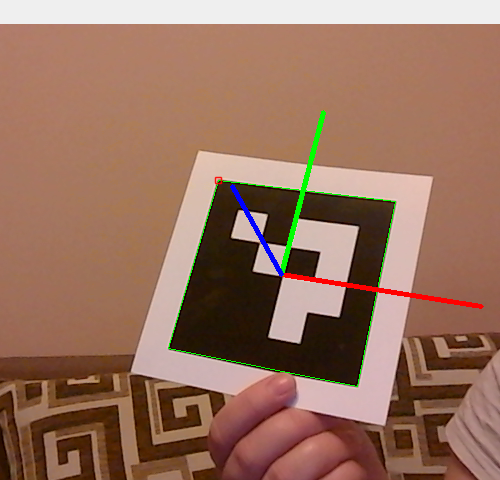
\includegraphics[scale=0.6]{images/felismeres_aruco.png}
	\caption{A demó eredménye}
	\label{fig:felismeres_aruco}
\end{figure}

\SubSection{A marker felismerésére készített program tesztje}

A végső programban az ArUco marker felismerés egy olyan függvényként jelenik meg, ami megkap egy képet és ha talál rajta markert, akkor visszaadja a megfelelő vektorokat (elforgatás és eltolás vektorokkal).

Ezen programrésznek a tesztelésére készítettem a nyomtatott markeremről képeket, és megnéztem milyen eredményeket ad vissza és felismeri-e a képen szereplő markert.

Azon kijelentés, hogy ha takarásba kerül a marker bármely része, akkor nem lesz továbbá felismerhető teljesen helytálló, mivel a program nem találta meg a markert, hogy ha annak egy aránylag kis része már ki volt takarva.

A programban az eredményt a vektorokat a fent már említett \texttt{estimatePoseSingle} \texttt{Markers} adja vissza.

Az \texttt{rvec} a marker kamerához képest vett elfordulása az $x$, $y$ és $z$ tengelyeken, a \texttt{tvec} pedig a marker eltolása ugyanezekhez. Tehát egy markerhez két vektorhármast kapunk vissza.

Ezen vektorok fogják a későbbiekben meghatározni a kirajzolandó modellek helyét a térben.

A lentebb szereplő képekhez kapott értékek közül néhány:
\begin{itemize}
\item 1. kép \texttt{rvec} és \texttt{tvec} értékei::
\[[-0.00010618, -0.00181233, 0.04695004]\]
\[[ 1.91320312, -1.6522394,  0.60923043]\]
\item 2. kép \texttt{rvec} és \texttt{tvec} értékei::
\[[-0.00082155,  0.00022395,  0.06280824]\]
\[[ 1.83895896, -1.46640971,  0.69940467]\]
\item 3. kép \texttt{rvec} és \texttt{tvec} értékei:
\[[-0.00619668, 0.00013297,  0.04769506]\]
\[[ 1.87260078 -1.66750728  0.64313328]\]
\item 5. kép \texttt{rvec} és \texttt{tvec} értékei:
\[-0.00501719, -0.01433891,  0.08986719]\]
\[[ 1.25084371,  2.11521712, -1.07834937]\]
\end{itemize}

Látható például, hogy az 5. kép eltolási és forgatási vektorainak értéke nagyobb, mint a 1. vagy 2., hisz ez messzebb van a képen a kamerához képest és jobban el van forgatva, mint a másik kettő.
Természetesen ha nem ismeri fel a amerkert, vagy nincs marker a képen 0 értéket add vissza a program.

\Aref{fig:detect}. ábrán láthatunk olyan képeket, amelyeknél sikeres volt a marker detektálása, \aref{fig:not_detect}. ábrán pedig olyanokat, amelyre sikertelen.

\begin{figure}[htp]
    \centering
   	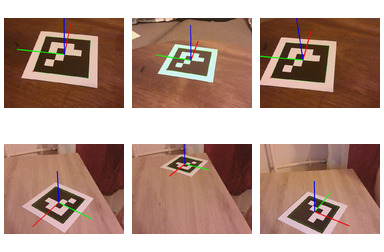
\includegraphics[width=\textwidth]{images/detect.jpg}
	\caption{Sikeres detektálás}
	\label{fig:detect}
\end{figure}

\begin{figure}[htp]
    \centering
   	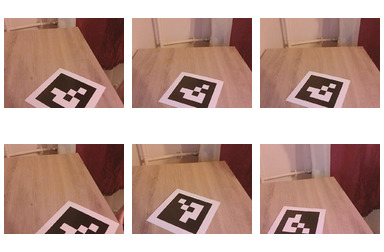
\includegraphics[width=\textwidth]{images/not_detect.jpg}
	\caption{Sikertelen detektálás}
	\label{fig:not_detect}
\end{figure}
